\section{Pruebas y Ensayos} \label{ensayos}
\AddToShipoutPictureBG*{
\includegraphics[width=\paperwidth,height=\paperheight]{Imagenes/Fondo Capitulo 5.pdf}}
\thispagestyle{plain}

\vspace{0.5cm}

\Large\scshape
\begin{center}
    {\Medium Relevamiento experimental del funcionamiento de\\ la plataforma resultante}
\end{center}
\normalfont
%\normalsize

\divider

Para darle cierre a este proyecto, con la plataforma ya diseñada e implementada exitosamente en la placa de circuito impreso, y todos sus componentes soldados, se avanzó con una serie de pruebas y ensayos para comprobar el diseño que se desarrolló. Estas son pruebas apuntadas a verificar que las distintas partes del sistema funcionen de la manera que fueron diseñadas.\\

\begin{figure}[h]
    \centering
    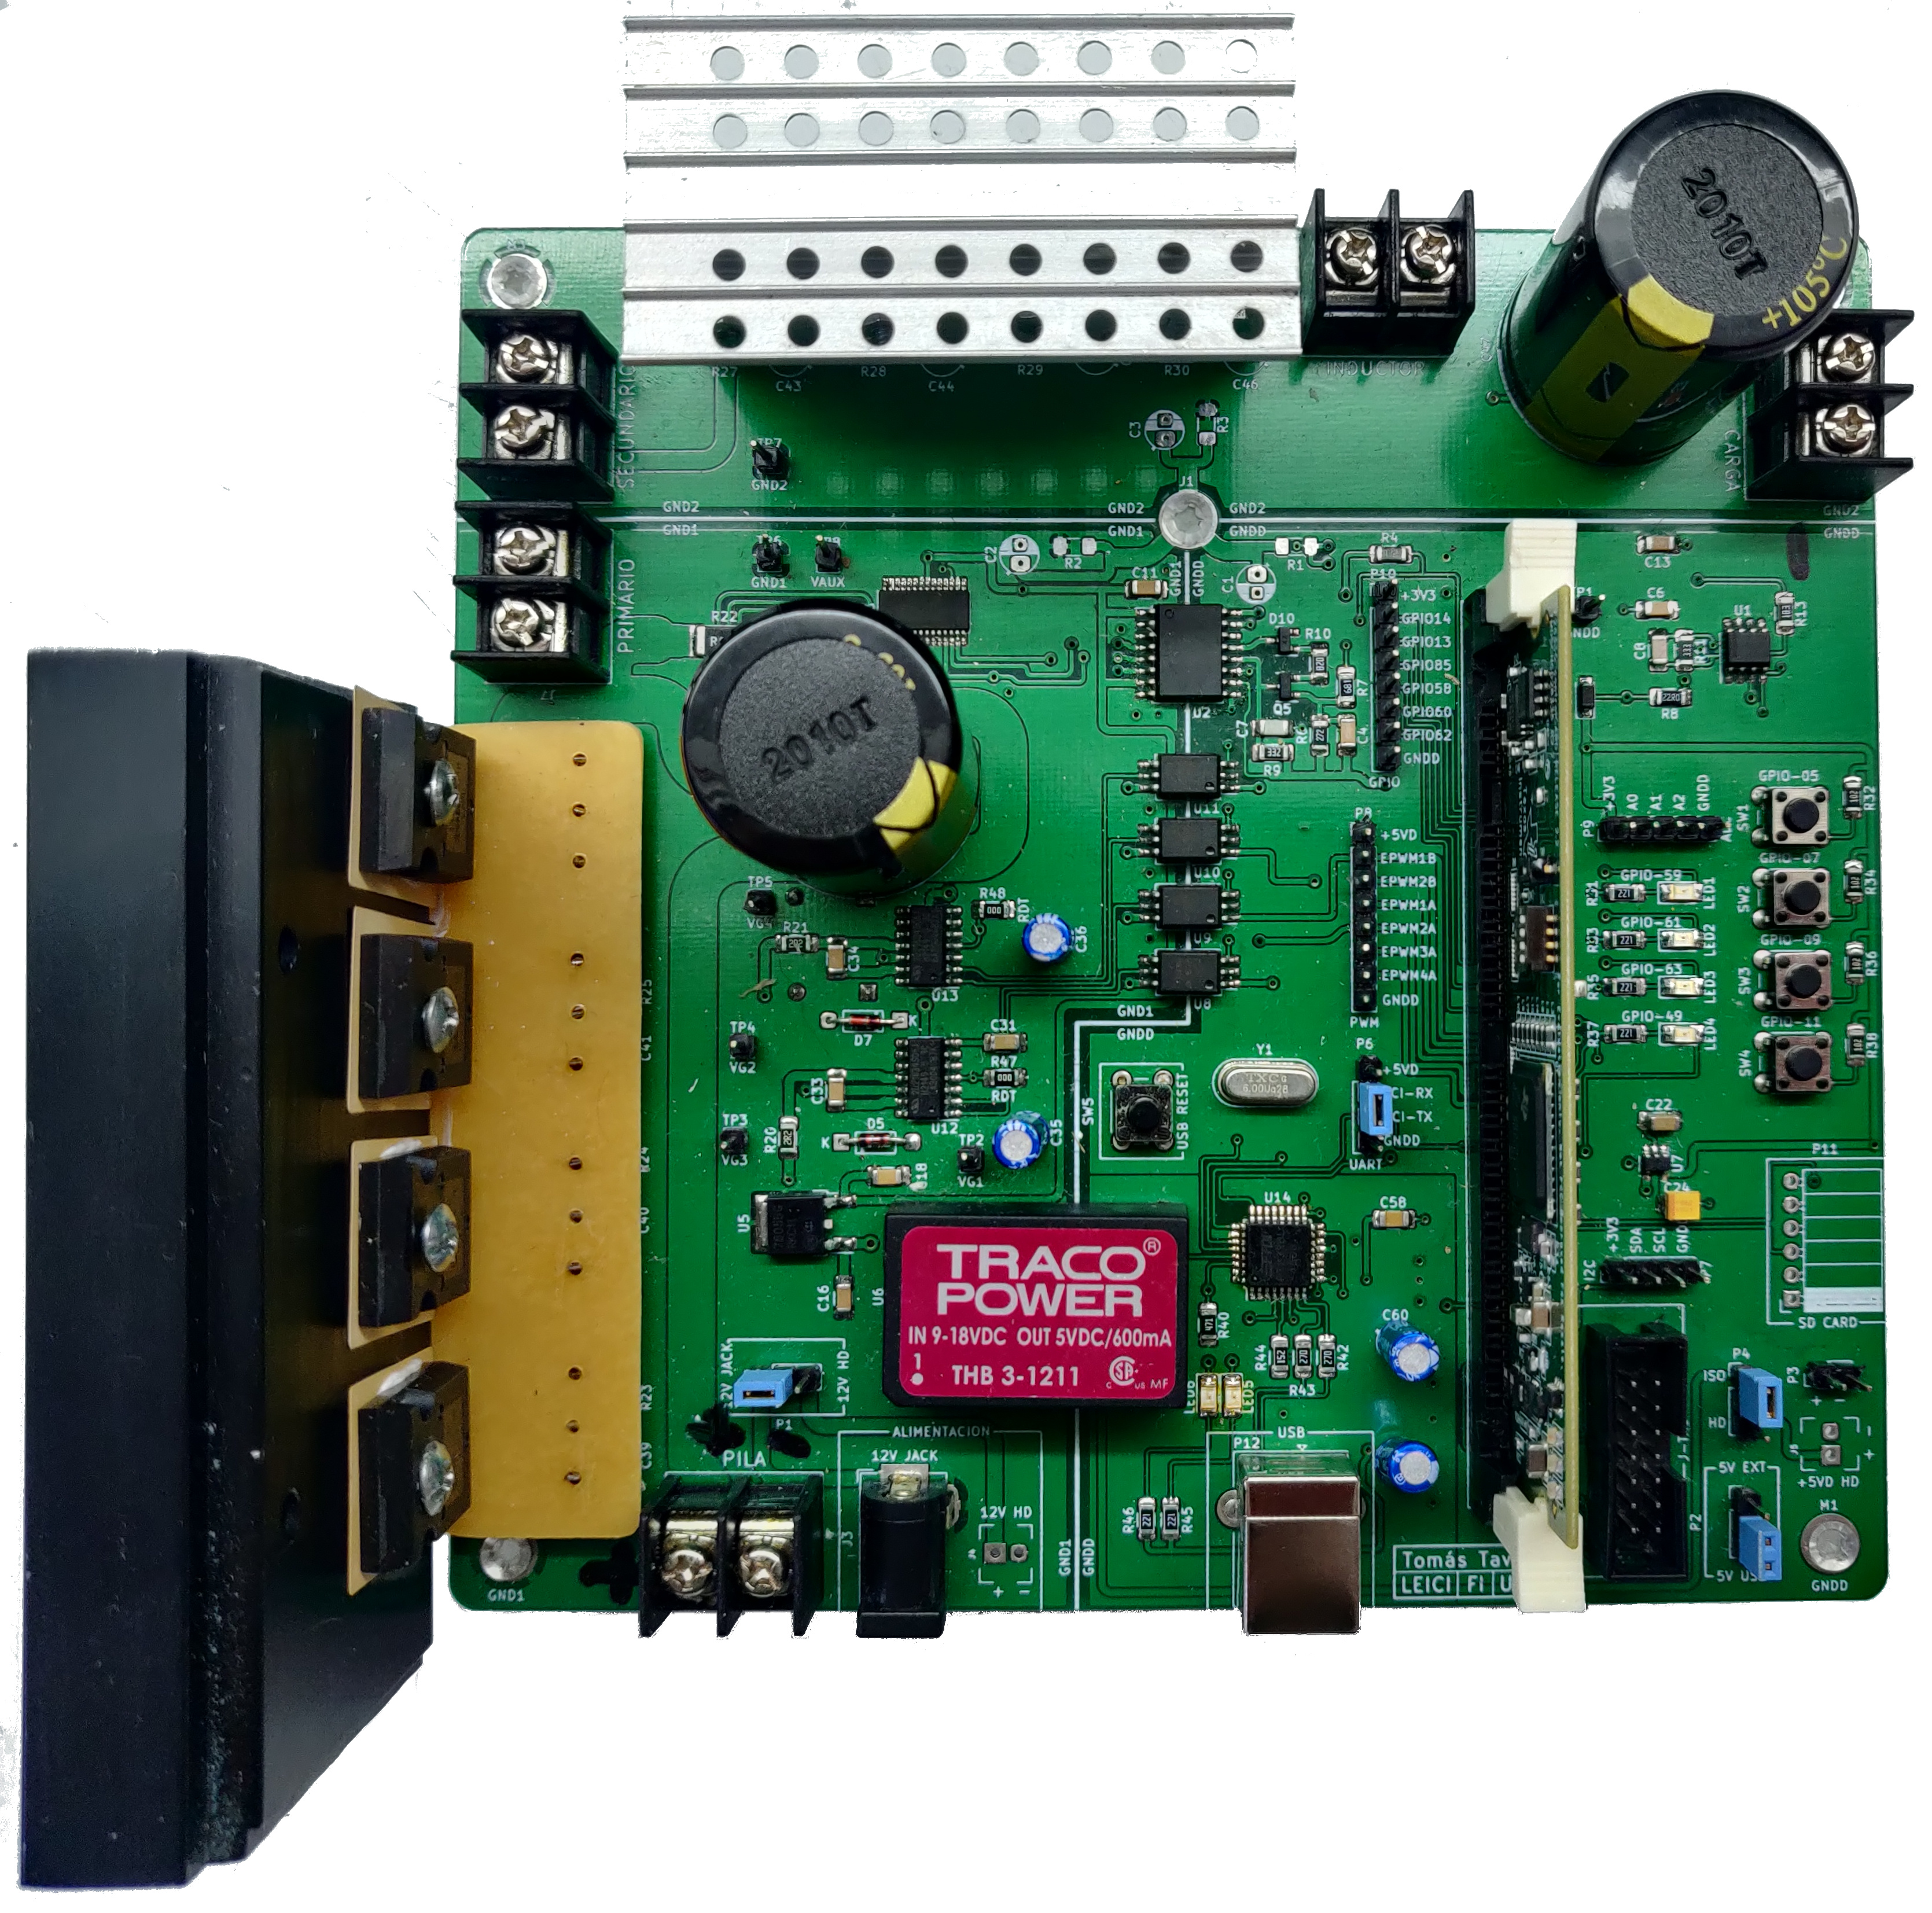
\includegraphics[scale=0.1]{Imagenes/Placa Final.jpg}
    \caption{La plataforma de evaluación en su estado final. Se puede ver el puente de MOSFET montado sobre la placa adaptadora a la izquierda, el rectificador en la parte superior, ocultado por el disipador, y la controlCARD en su socket a la derecha.}
    \label{plataforma_completa}
\end{figure}

Por limitaciones de tiempo, no se pudieron hacer las pruebas de todos los componentes: se realizaron pruebas del módulo de generación de ondas PWM, del circuito driver para el disparo de las llaves, y finalmente una evaluación del convertidor CC-CC puente completo para distintas condiciones de carga. Con el éxito de estos ensayos, también se demostró indirectamente el funcionamiento satisfactorio de todos los circuitos de alimentación y del controlador digital de señales.\\

\subsection{Configuración Experimental}

Para realizar todos los ensayos, se utilizó como instrumento de medición un osciloscopio digital doble canal Tektronix TBS1102B de \SI[]{100}{\mega\hertz} de ancho de banda y 2 GS/s, tal como el que se observa en la figura \ref{test_setup}. Para alimentar la tensión y corriente de entrada al convertidor, se utilizó una fuente de laboratorio de corriente continua HP 6010A, visible en la esquina superior derecha de la imagen, con capacidad de hasta \SI[]{200}{\volt}, \SI[]{17}{\ampere} y \SI[]{1000}{\watt}. Finalmente, para simular las condiciones de carga a la salida de la plataforma, se utilizo la carga electrónica variable ITECH I8514B+ que se mencionó en el capítulo \ref{analisis}, presente en la figura debajo de la fuente de laboratorio.\\

\begin{figure}[h]
    \centering
    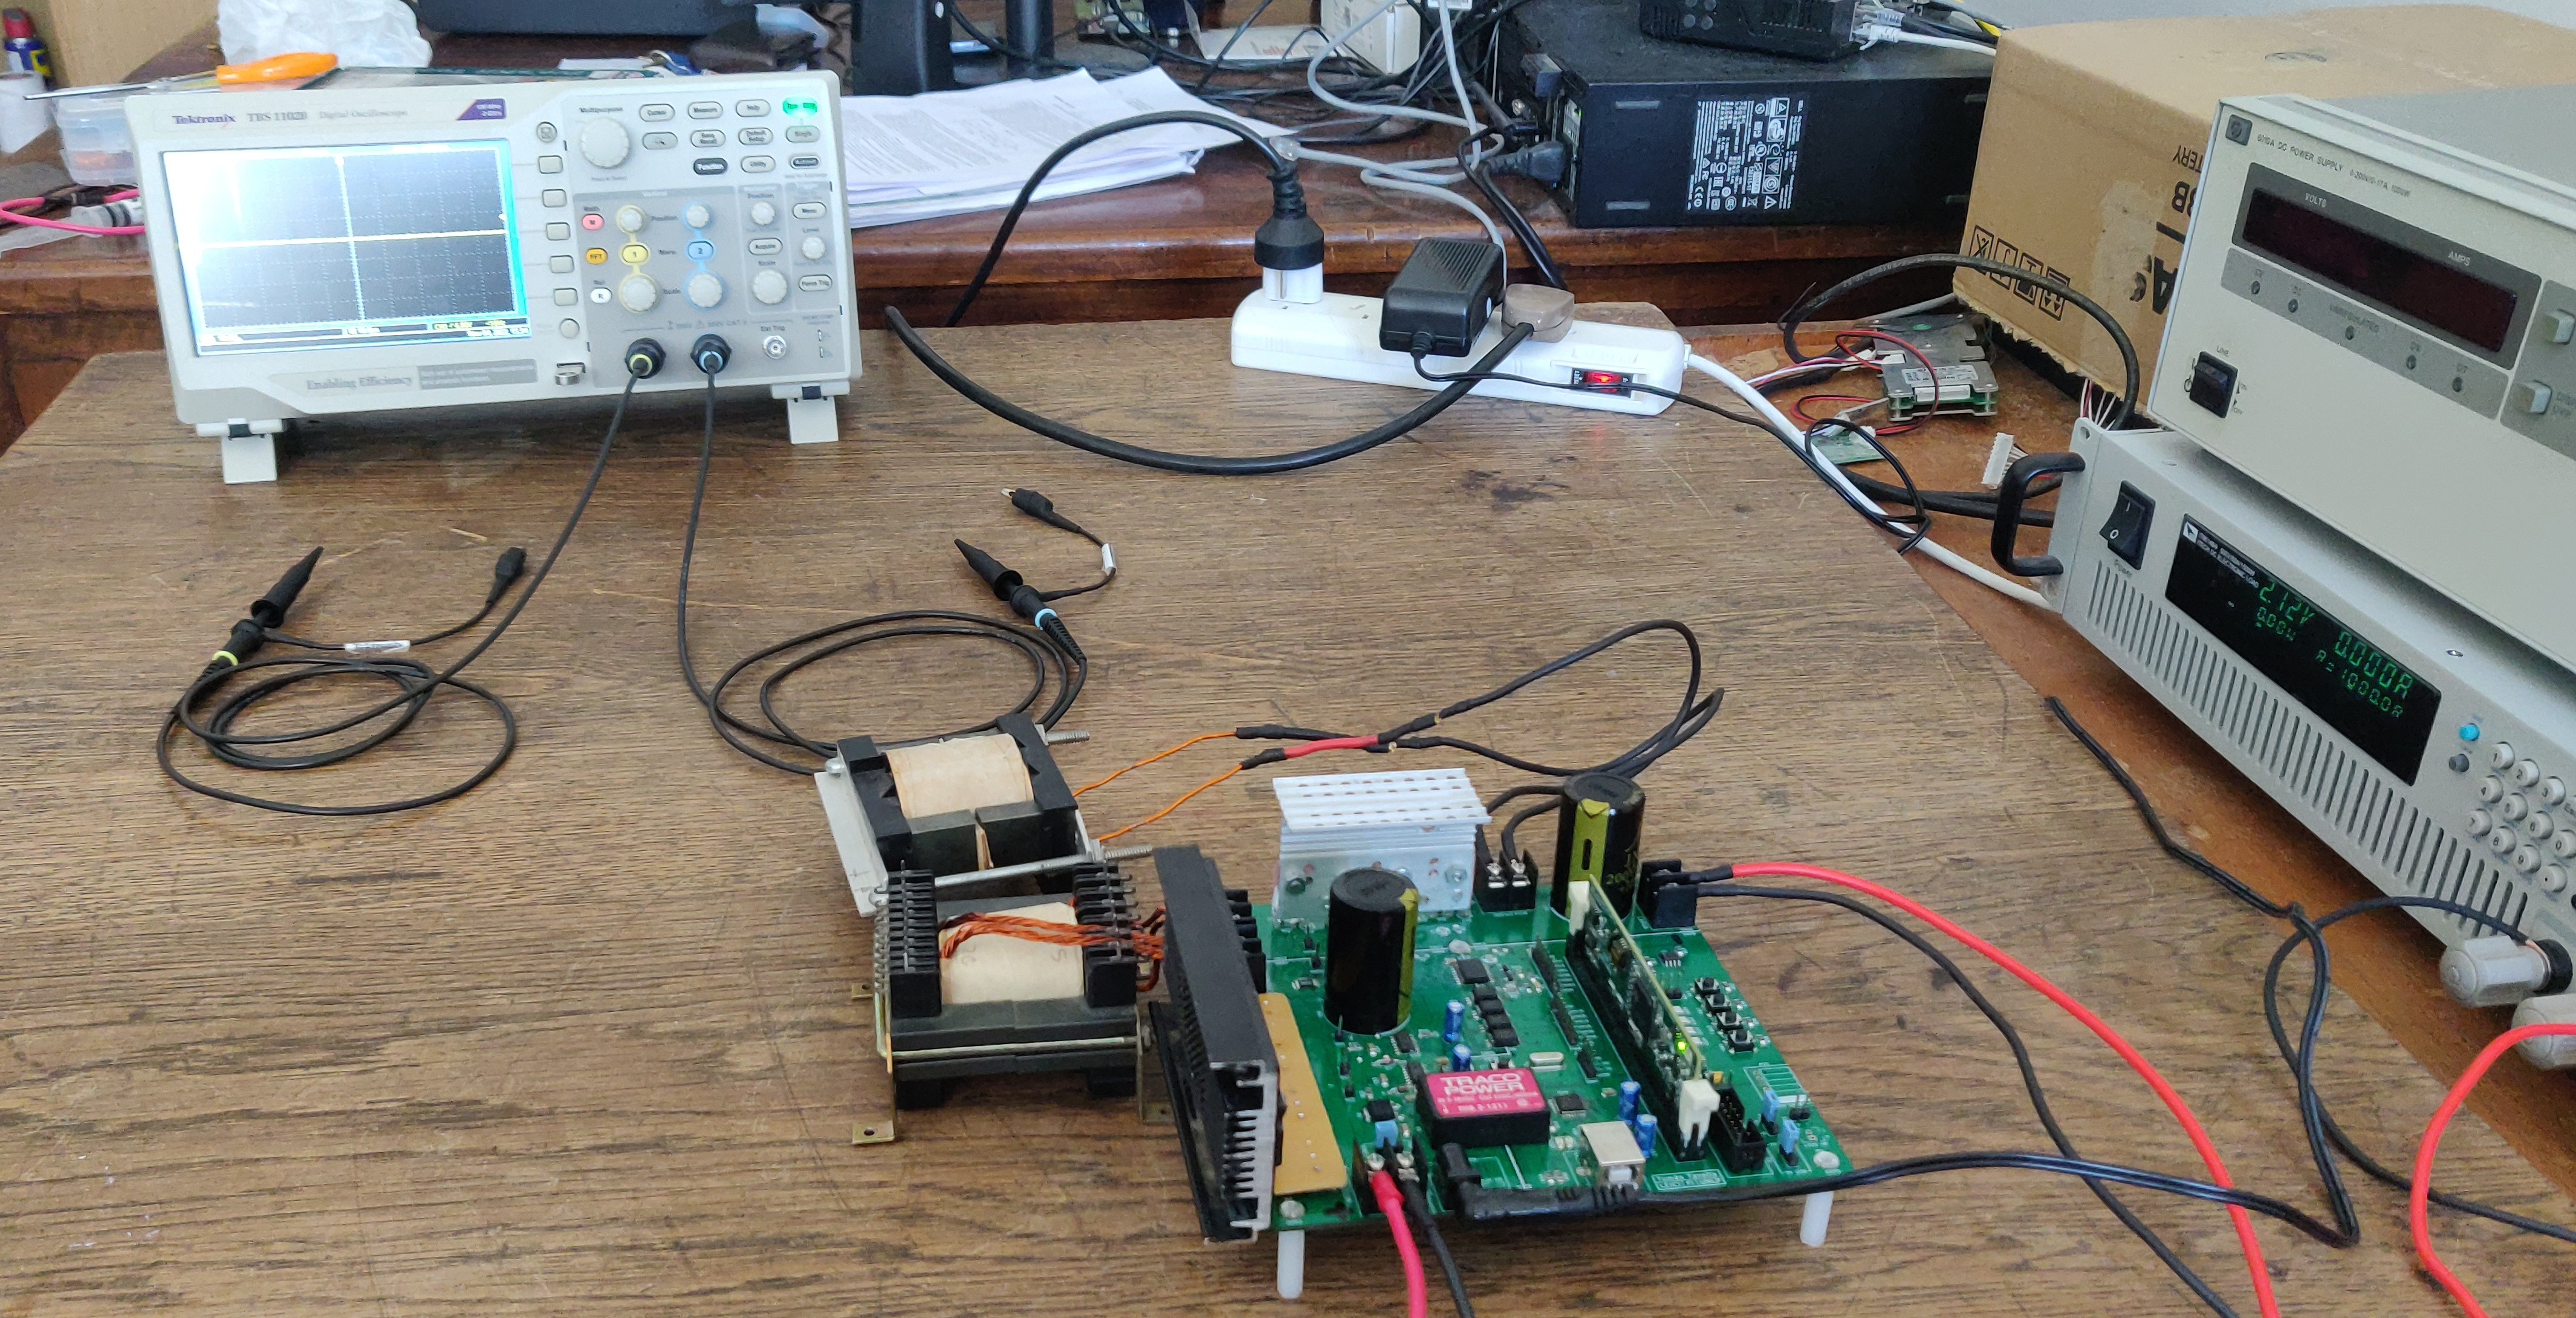
\includegraphics[scale=0.09]{Imagenes/Setup Ensayo.jpg}
    \caption{Setup utilizado para la realización de los ensayos de evaluación del convertidor CC-CC puente completo.}
    \label{test_setup}
\end{figure}

Para poder realizar todas las pruebas, también fue necesaria la programación de un firmware mínimo que pusiera en funcionamiento los módulos ePWM necesarios para generar las señales de comando, que luego son enviadas a los circuitos driver y generan la excitación del puente de MOSFET. Además, se agregó un código que, mediante interrupciones externas, varía el ciclo de trabajo mediante el accionamiento de dos pulsadores, y genera una indicación del mismo utilizando cuatro LEDs.\\

Este firmware se programó en lenguaje C, utilizando el IDE provisto por Texas Instruments, llamado \textit{Code Composer Studio} (CCS), que incluye un compilador, bibliotecas y las herramientas de software necesarias para cargar los programas al controlador. Como la carga y debugging del firmware se realiza a través del puerto JTAG, se utiliza una \textit{docking station} para el controlador, provista por Texas Instruments, que cuenta con la capacidad de emular la funcionalidad de JTAG a través de USB, y actúa como intermediario entre el puerto USB de la computadora y el puerto JTAG de la plataforma.\\ 

\begin{figure}[h]
    \centering
    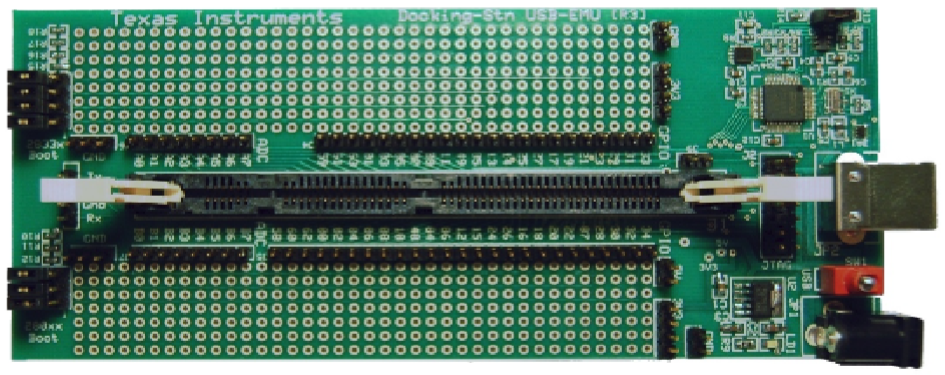
\includegraphics[scale=0.25]{Imagenes/Docking Station.png}
    \caption{Docking station para controlCARD de la serie C2000, con el puerto USB y JTAG a la derecha.}
    \label{docking_station}
\end{figure}

\newpage

\subsection{Ensayo sin Carga}

Como primer ensayo, se realizaron mediciones de la tensión en el bobinado primario $V_p$, junto con las tensiones del punto medio de cada pata del puente de transistores, $V_p^+$ y $V_p^-$. Todas estas pruebas se realizaron con distintos niveles de desfase entre las señales de las patas del puente, que son equivalentes a distintos valores de ciclo de trabajo del secundario $D_{sec}$.\\

Los terminales de entrada correspondientes a la pila de combustible fueron conectados a la fuente de laboratorio HP6010A, entregando una tensión continua de \SI{30}{\volt}. Sin embargo, como esta fue la primer prueba realizada sobre el convertidor CC-CC, se llevó a cabo sin ningún tipo de carga, dejando los terminales correspondientes a ambos bobinados del transformador a circuito abierto. De esta manera, no existe circulación de corriente, y no se corre el riesgo de destruir algún componente en caso de una falla inesperada del circuito, como podría ser un cortocircuito.\\

El objetivo de este ensayo es relevar el correcto funcionamiento de los circuitos de excitación del puente, compuestos por los dos drivers 2ED21834-S06J. Se debe verificar que sean capaces de disparar los IRFP150, y que funcionen correctamente los circuitos de bootstrap necesarios para activar los transistores del lado alto.\\

\subsubsection{Resultados}

\begin{figure}[h]
    \centering
    \hspace{0.5em}
    \begin{subfigure}{0.47\textwidth}
        \centering
        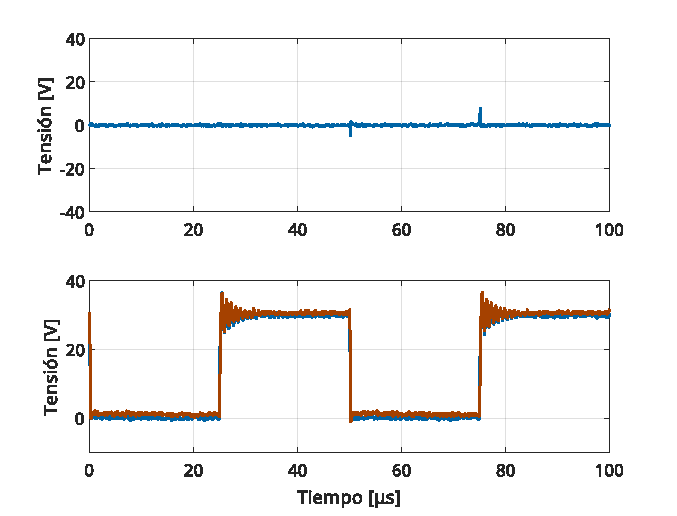
\includegraphics[width=\textwidth]{Imagenes/Sin Carga - Fase 0.pdf}
        \caption{Fase relativa de 0°.}
        \label{fig:ensayo_sincarga0}
    \end{subfigure}
    \hspace{0.5em}
    \begin{subfigure}{0.47\textwidth}
        \centering
        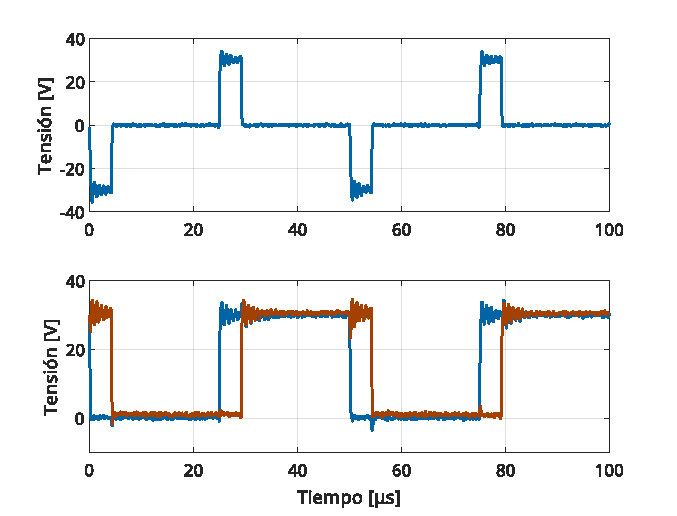
\includegraphics[width=\textwidth]{Imagenes/Sin Carga - Fase 30.pdf}
        \caption{Fase relativa de 30°.}
        \label{fig:ensayo_sincarga30}
    \end{subfigure}
    \hfill\vspace{1em}
    \begin{subfigure}{0.47\textwidth}
        \centering
        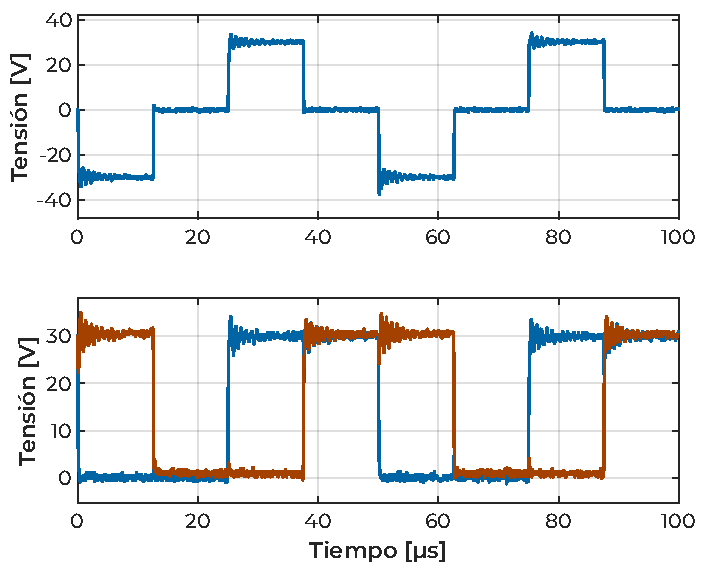
\includegraphics[width=\textwidth]{Imagenes/Sin Carga - Fase 90.pdf}
        \caption{Fase relativa de 90°.}
        \label{fig:ensayo_sincarga90}
    \end{subfigure}
    \hspace{0.5em}
    \begin{subfigure}{0.47\textwidth}
        \centering
        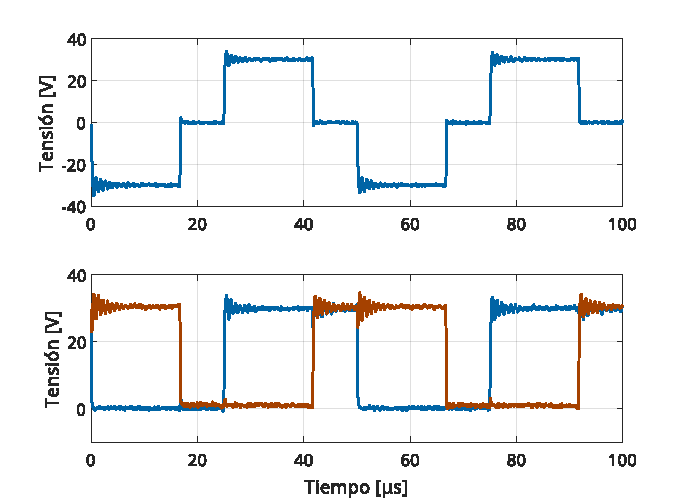
\includegraphics[width=\textwidth]{Imagenes/Sin Carga - Fase 120.pdf}
        \caption{Fase relativa de 120°.}
        \label{fig:ensayo_sincarga120}
    \end{subfigure}
    \caption{Resultados de la medición de tensión de bobinado primario $V_p$ y tensiones de medios puentes $V_p^+$ y $V_p^-$.}
    \label{fig:ensayo_sincarga}
\end{figure}

Se pueden observar en la figura \ref{fig:ensayo_sincarga} las señales de tensión de bobinado primario y de ambos medios puentes medidas con el osciloscopio durante la realización del ensayo. Las señales de tensión de los medios puentes consisten en ondas cuadradas de \SI[]{20}{\kilo\hertz} de frecuencia fundamental y ciclo de trabajo $D$ fijo de 50\%, mientras que como tensión del bobinado se toma la diferencia de ambas ondas cuadradas. Así, entonces, se produce la forma de tensión \quotes{escalonada} y bipolar, comúnmente llamada onda cuadrada modificada, que se ve en las figuras \ref{fig:ensayo_sincarga30}, \ref{fig:ensayo_sincarga90} y \ref{fig:ensayo_sincarga120}.\\

Este ensayo generó resultados satisfactorios, ya que las ondas cuadradas del medio puente y la onda cuadrada modificada del primario se pueden ver claramente, con flancos de subida y bajada bien definidos y tiempos de establecimiento casi imperceptibles frente al período de \SI[]{50}{\micro\second}. Esto nos indica que el circuito de excitación está funcionando correctamente, y es capaz de disparar rápida y efectivamente a los transistores.\\

Sin embargo, en la figura se pueden notar artefactos de \textit{ringing} en todos los flancos de subida de las señales: fenómenos transitorios con oscilaciones de alta frecuencia que se suelen presentar a la hora de conmutar una llave por la que circulan grandes corrientes (y en líneas generales para sistemas de banda limitada). Estas oscilaciones consumen energía que de otra manera hubiese llegado a la salida del convertidor, reduciendo la eficiencia energética total del sistema. Además, generan sobrepicos de tensión sobre las llaves que, en casos extremos, pueden llegar a dañarlas o destruirlas.\\

Se puede ver también como este efecto se transmite por acoplamiento e interferencia electromagnética: cuando una de las ondas cuadradas tiene un flanco de subida, se puede ver una oscilación similar inducida en la otra señal cuadrada. En cualquier caso, la presencia del ringing en el caso de este ensayo no es de mayor preocupación, ya que los sobrepicos de tensión que genera son baja magnitud, de alrededor de \SI[]{7}{\volt} por encima de los \SI{30}{\volt} finales de la onda cuadrada, o alrededor del 23\%.\\

Habiendo obtenido un resultado exitoso del primer ensayo, se puede pasar al ensayo con carga, dónde se va a poder observar y evaluar el funcionamiento del convertidor completo en condiciones de carga moderadas, incluyendo transformación y rectificación de la tensión del bobinado primario.\\

\newpage

\subsection{Ensayo con Carga}

Una vez realizado el ensayo sin carga, y verificado el funcionamiento sin fallas del puente de transistores, se puede proceder a la siguiente prueba. A diferencia del caso anterior, se va a ensayar el convertidor CC-CC completo, conectando el transformador y el inductor de salida $L_f$ a sus terminales correspondientes (ver figura \ref{test_setup}).\\

Como ya se mencionó, la fuente de laboratorio HP 6010A está encargada de proveer la corriente y tensión necesaria en el primario, mientras que la carga electrónica variable ITECH IT8514B+ se conecta en el terminal de salida del secundario y absorbe la corriente continua de la salida. La fuente se configuró en modo de tensión constante (operando a \SI[]{15}{\volt} o \SI[]{30}{\volt}) con limitador de corriente variable, y la carga electrónica en modo de resistencia constante.\\

En esta serie de ensayos se miden distintas variables representativas del sistema: tensión de salida $V_{out}$, tensión rectificada $V_{rect}$, corriente de salida $I_{out}$, corriente en el inductor $I_{Lf}$ y tensión del secundario $V_s$. Como en este caso va a existir circulación de corriente, incluso llegando a cargas cercanas a los \SI[]{100}{\watt} (un tercio de la máxima potencia del sistema), se va a poder observar como se comporta la plataforma frente a grandes circulaciones de corriente, incluido el funcionamiento del rectificador de diodos que no fue evaluado en las pruebas sin carga.\\

\subsubsection{Pruebas a 15 V}

Para proteger a los componentes, se comenzaron los ensayos con la fuente de laboratorio entregando una tensión continua de \SI[]{15}{\volt}, limitando la máxima tensión y corriente que cae sobre las llaves y diodos rectificadores.

\begin{figure}[h]
    \centering
    %\hspace{0.5em}
    \begin{subfigure}{0.48\textwidth}
        \centering
        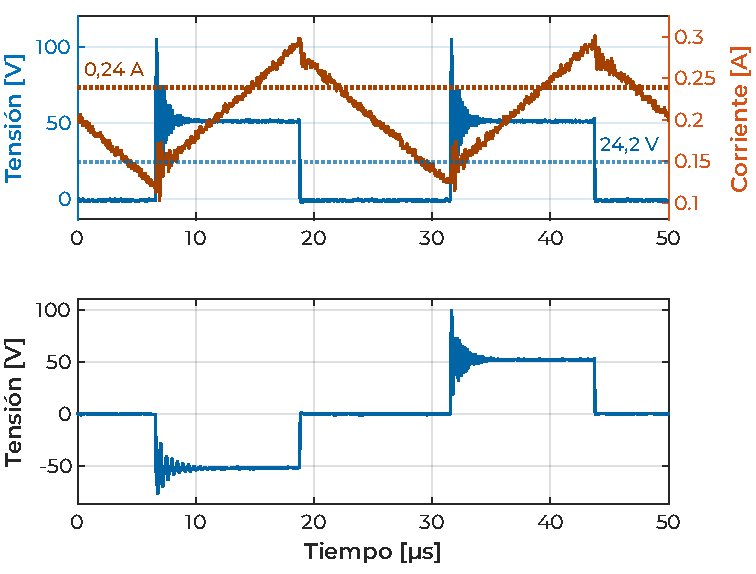
\includegraphics[width=\textwidth]{Imagenes/Con Carga - Caso 1.pdf}
        \caption{Ciclo de trabajo de 50\%.}
        \label{fig:ensayo_concarga15V_1}
    \end{subfigure}
    \hspace{0.5em}
    \begin{subfigure}{0.48\textwidth}
        \centering
        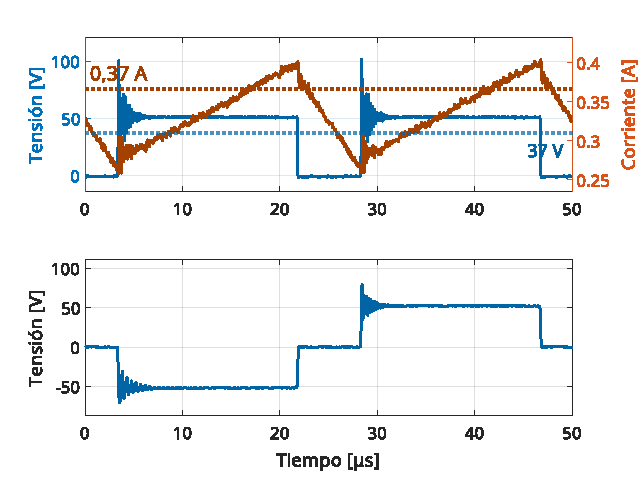
\includegraphics[width=\textwidth]{Imagenes/Con Carga - Caso 5.pdf}
        \caption{Ciclo de trabajo de 75\%.}
        \label{fig:ensayo_concarga15V_2}
    \end{subfigure}
    \caption{Tensión rectificada $V_{rect}$, corriente de inductor $I_{Lf}$ y tensión del bobinado secundario $V_{sec}$ para una carga de \SI[]{100}{\ohm} a la salida.}
    \label{fig:ensayo_concarga15V}
\end{figure}

\begin{figure}[h]
    \centering
    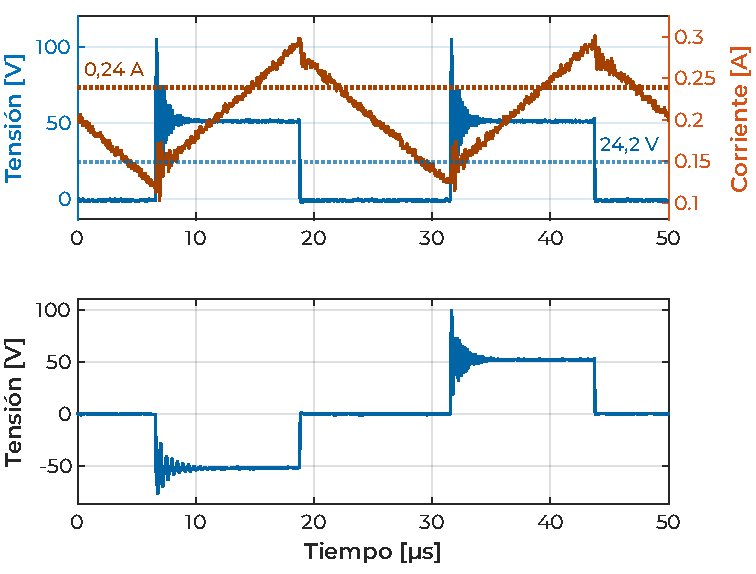
\includegraphics[scale=1]{Imagenes/Con Carga - Caso 1.pdf}
    \caption{Tensión rectificada $V_{rect}$ y corriente de inductor $I_{Lf}$ para una carga de \SI[]{100}{\ohm}, ciclo de trabajo de 50\% y tensión de entrada de \SI[]{15}{\volt}.}
    \label{ConCargaI}
\end{figure}

\lipsum[3]\\

\afterpage{\blankpage}\newpage